\documentclass[12pt,a4paper]{article}
\usepackage{rmpackages}																% usual packages
\usepackage{rmtemplate}																% graphic charter
\usepackage{rmexocptce}																% for DS with cptce eval

%\cfoot{} 													% if no page number is needed
%\renewcommand\arraystretch{1.5}		% stretch table line height

\newcommand{\ritem}{\refstepcounter{enumi}\item[\color{bleu_f}\textbf{\theenumi .}]}

\begin{document}

\begin{header}
TP

Un diapason électronique
\end{header}

Les \textbf{micro-contrôleurs} sont des circuits intégrés qui regroupent les fonctions essentielles d'un ordinateur.
Il permettent de réaliser de nombreux systèmes électroniques.

L'objectif de la séance est de réaliser un diapason électronique avec une carte Arduino.
Il s'agit d'une carte programmable équipée d'un micro-contrôleur : grâce à plusieurs entrées et sorties il est possible d'analyser les informations issues de différents \textbf{capteurs} (microphone, photodiode, thermomètre, etc.) et de contrôler des \textbf{actionneurs} (haut-parleur, LED, moteur, etc.).

Pour donner des instructions à la carte, on utilise le langage Arduino.

\section*{Premiers pas}

Les programmes utiles pour le TP sont dans le dossier \og Ordinateur \textrightarrow{} Ma classe \textrightarrow{} Documents en consultation \textrightarrow{} Physique-Chimie \textrightarrow{} TP Arduino \fg{}.
\begin{enumerate}
\item \rea{}

Copier-coller tout le dossier \og TP Arduino \fg{}  dans votre espace de travail personnel où vous pourrez modifier les fichiers.
\end{enumerate}

\begin{center}
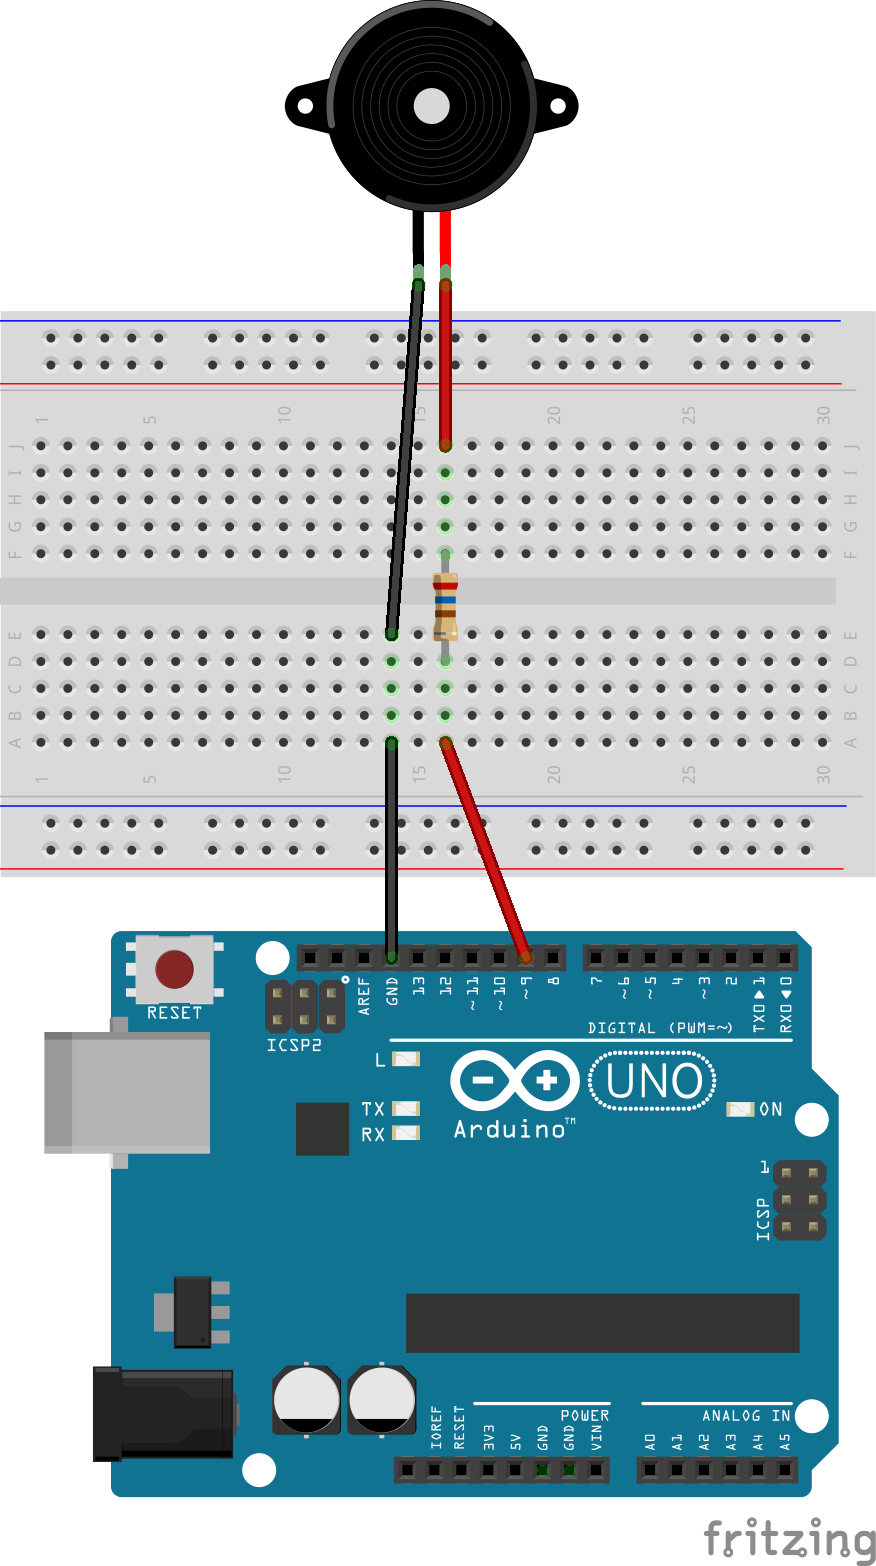
\includegraphics[scale=1, angle=-90]{fritzing/buzzer_bb.png}
\end{center}

\begin{enumerate}[resume]
\item \rea{}

Réaliser le montage électronique schématisé ci-dessus avec le matériel à votre disposition.

\item \rea{}

Connecter la carte à l'ordinateur avec le câble USB.
Ouvrir le programme \texttt{programme1} avec le logiciel Arduino.
Dans l'onglet \og Outil \fg{}, vérifier que le type de carte sélectionné est bien Arduino Uno et que le port sélectionné est bien COM1.

\ritem \rea{} \com{}

Compiler le programme et l'envoyer vers la carte en cliquant sur 
\includegraphics[height=0.75\baselineskip]{images/arduino_televerser.png} Téléverser.
Décrire succinctement ce qu'il se passe après le téléversement.

\appelprof{\rea{} : Appelez le professeur pour lui présenter votre montage.}
\end{enumerate}

\section*{La commande \texttt{tone}}

La carte exécute le programme envoyé dès qu'elle le reçoit, puis à chaque fois qu'elle est rallumée, soit en appuyant sur le bouton RESET de la carte ou lorsqu'on la connecte à nouveau en USB.

Un programme Arduino comprend au minimum deux fonctions (\texttt{setup} et \texttt{loop}) qui peuvent contenir plusieurs commandes.

\begin{lstlisting}[style=Arduino]
// fonction d'initialisation de la carte
void setup() {
  pinMode(9, OUTPUT); // 9ème broche de la carte en mode sortie
  tone(9, 440, 1000); // fonction générant un signal périodique
}
\end{lstlisting}

\begin{enumerate}[resume]
\ritem \anarai{}
\label{quest:tone}

À la ligne 4 du \texttt{programme1}, la commande \texttt{tone} comprend trois arguments (trois nombres) séparés par des virgules.
À votre avis, à quoi correspond chacun de ces arguments ?

\ritem \anarai{}
\label{quest:tone_protocole}

Comment pourrait-on vérifier la réponse à la question précédente ?
% Élaborer un protocole permettant de vérifier vos hypothèses.

\appelprof{\anarai{} : Appelez le professeur pour lui présenter votre protocole.}

\ritem \rea{} \val{}

Vérifier la réponse de la question \ref{quest:tone}.
Votre réponse était-elle correcte ?
Sinon, indiquez à quoi correspondent les trois arguments.
% Mettre en place le protocole pour vérifier vos hypothèses.

\ritem \app{} \anarai{}

Comparer les programmes \texttt{programme1} et \texttt{programme2}.
Pourquoi la fonction \texttt{loop} s'appelle-t-elle ainsi ?
\end{enumerate}

\section*{Construire un diapason électronique}

Les broches 2 à 13 de l'Arduino peuvent servir de sorties \textbf{digitales}, c'est-à-dire que ces broches ne permettent d'obtenir que des tensions de \unit{0}{V} (LOW : état bas) ou \unit{5}{V} (HIGH : état haut).
La broche 13 de l'Arduino est de plus connectée à une LED située à côté (L).
Tant qu'elle est allumée, la broche 13 est dans l'état haut et tant qu'elle est éteinte, la broche est dans l'état bas.

\begin{enumerate}[resume]
\ritem \rea{} \app{}

Téléverser le \texttt{programme3} et observer ce qu'il se passe. 
Comment traduiriez-vous la commande \texttt{delay} des lignes 9 et 11 du \texttt{programme3} ?
 
\ritem \anarai{} \rea{}

Représenter l'allure du signal obtenu en sortie de la broche 13 en fonction du temps.
Comment peut on qualifier ce signal ?
Quelle est sa période ?

\ritem \rea{}

Calculer la période $T$ d'un signal de fréquence $f = \unit{440}{Hz}$.

\ritem \app{} \anarai{} \rea{} \val{}

Modifier le \texttt{programme3} et éventuellement votre montage électronique pour réaliser un diapason électronique (sans utiliser la commande \texttt{tone}).

\appelprof{\val{} : Appeler le professeur quand votre diapason électronique fonctionne ou en cas de difficulté.}


\end{enumerate}

\end{document}